\section{Preliminary}
\label{sec:preliminary}

\begin{figure}[h]
	\centering
	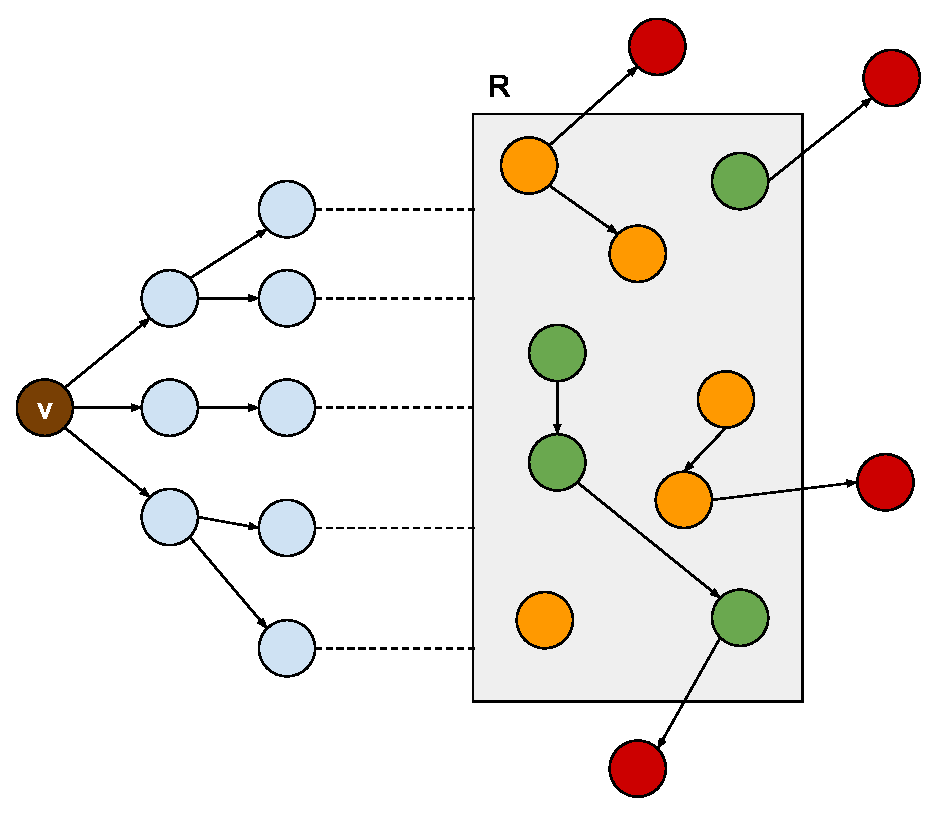
\includegraphics[width=0.88\linewidth]{images/image10.eps}
	\caption{A social graph showing friend-friend connections and also the region of interest}
	\label{fig:socio-spatial-graph}
\end{figure}

{\bf Graph Data.} A weighted directed graph $G=(V,E,S)$ consists of (1) a set of vertices $V$; (2) a set of directed edges $E\subset V\times V$ with weights. If $(u,v)\in E$, there exists one edge from vertex $u$ to $v$; (3) a function $S$ defined on $V$ that decides spatial attribute of a given vertex. $S(v)$ returns spatial property of $v$ (denoted as $v.spatial$) and the value will be null when $v$ brings no spatial attribute. $S(v)$ can be a geometrical a point, line, or polygon. For ease of presentation, we assume that a spatial attribute of spatial vertex is represented by a point.
%${\GeoReach} deals with a directed property graph $G=(V,E)$ where (1)~$V$ is a set of vertices such that each vertex has a set of properties (attributes) and (2)~$E$ is a set of edges in which every edge can be represented as a tuple of two vertices $v_1$ and $v_2$ ($v_1,v_2\in V$). The set of spatial vertices $V_S \subseteq V$ such that each $v \in V_{S}$ has a spatial attribute (property) $v.spatial$. The spatial attribute $v.spatial$ may be a geometrical point, rectangle, or a polygon. For ease of presentation, we assume that a spatial attribute of spatial vertex is represented by a point. Figure~\ref{fig:graph_example} depicts an example of a directed property graph. Spatial Vertices $V_S$ are represented by black colored circles and are located in a two-dimensional planer space while white colored circles represent regular vertices that do not possess a spatial attribute. Arrows indicate directions of edges in the graph.

\textbf{Path and Shortest Path.} A path is a sequence of vertices and edges that are distinct from one another. A path is denoted as $p =$ ($v_1$, $e_1$,..., $v_{n-1}$, $e_{n-1}$, $v_n$) where $v_i\neq v_j~and~e_i\neq e_j (i\neq j)$. Length of $p$ is denoted as $L(p) = \sum\limits_{i = 1}^{n-1}w(e_i)$. This path starts from vertex $v_1$ to $v_n$. In a weighted directed graph $G$, there possibly exists multiple paths between two vertices $u$ and $v$. $Paths(u,v) = \{p|p = (u,e_1,..., v)\}$ is to represent the set of all paths that start from $u$ and end at $v$. Shortest path between $u$ and $v$ is a path that has the shortest $L(p)$ where $p\in Paths(u,v)$, denoted as $ShortestPath(u,v)$.

\textbf{Shortest path between vertex and spatial region.} Given a vertex $v$ and a spatial region $R$, there exists many shortest paths between $v$ and each spatial vertex $u$ inside $R$, depending on how many spatial vertices are located in $R$. RangeReachShortestPath($v$, $R$, $k$) returns the $k$ shortest paths among all shortest paths between $v$ and $u$.

\iffalse
Given a graph $G(V, E)$ where,

\quad$V \rightarrow set\ of\ vertices$

\quad$E \rightarrow set\ of\ edges$

$Vs \subset V$ have spatial attributes; i.e. $\forall v \in Vs \Leftrightarrow v.spatial$ attribute exists\\


\textbf{RangeReachPaths S(G, v, R):} a set of shortest paths starting from v that reach a region R in graph G, where R is a spatial range predicate. Let's abbreviate this as RRP(v, R).

\textbf{Path, P(u, w):} A set of vertices along the way from u to w \(\Rightarrow w\ is\ reachable\ from\ u\)

\quad${P(u, w) \in S(v, R) \Leftrightarrow}$

\quad\quad{u = v and}

\quad\quad${w \in Vs}$ and

\quad\quad{w.spatial lies in region R}\\

\fi

Figure \ref{fig:socio-spatial-graph} pictorially represents the entire problem. v is the source vertex and R is the region of interest. Red, green and yellow vertices have spatial attributes like latitude and longitude information. Red vertices fall outside the region and so are not returned by RRP. Yellow vertices fall inside R but cannot be reached from v, so are not returned by RRP. Green vertices satisfy both these conditions as they fall inside the region and are also reachable from v. ~Therefore, RRP returns the paths to all green vertices. These paths with rich social information about the relationship with v, can be fed into a recommendation system which can rank them.

\iffalse
\begin{figure}[h]
    \centering
    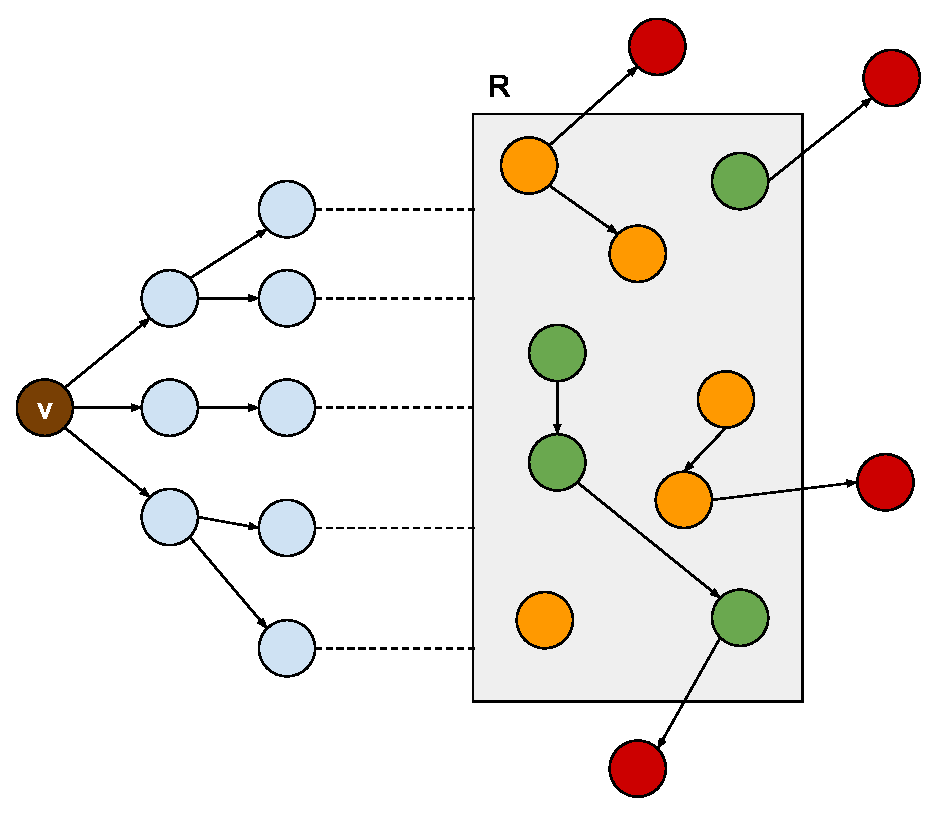
\includegraphics[width=0.5\linewidth]{images/image10.eps}
    \caption{A social graph showing friend-friend connections and also
the region of interest}
    \label{fig:socio-spatial-graph}
\end{figure}

Figure \ref{fig:socio-spatial-graph} pictorially represents the entire problem. v is the source vertex and R is the region of interest. Red, green and yellow vertices have spatial attributes like latitude and longitude information. Red vertices fall outside the region and so are not returned by RRP. Yellow vertices fall inside R but cannot be reached from v, so are not returned by RRP. Green vertices satisfy both these conditions as they fall inside the region and are also reachable from v. ~Therefore, RRP returns the paths to all green vertices. These paths with rich social information about the relationship with v, can be fed into a recommendation system which can rank them.
\fi